\chapter{序論}
\label{chap_intro}

% 英語で言うところのイントロダクションです。通常、「序論」(introduction)で始める場合は「結論」(conclusion)という章で締めます。もし「はじめに」で始まる場合は「おわりに」です。

% この章では研究の背景や課題などを簡潔に説明します。2から4ページもあれば十分ですし、細かく節に分ける必要もありません。この章で必要なことは、なぜこの論文が書かれたのか、過去の研究に対する位置付け・課題は何か、この研究でどこまでを明らかにしようとしているのかを少ないページ数で説明することです。

% このような序論の存在しない修士論文はたくさん存在しますが、何十ページにもなる修士論文では研究の位置付けや課題がどこに書かれているのか読者は見失いやすくなります。先頭に独立した章で簡潔に道筋を示すことで、続く章を読者が読みやすくなります。

\section{素粒子標準模型}
\label{sec_intro_sm}
素粒子標準模型は物質を構成する基本粒子である素粒子とそれらの間に働く相互作用を記述した理論体系である。標準模型を構成する素粒子は、物質を構成するフェルミオン、相互作用を媒介するゲージボゾン、質量の起源となるヒッグス粒子に分けられる。
表\ref{tab:fermion}にフェルミオンの性質をまとめる。フェルミオンは強い相互作用をしないレプトンと、強い相互作用をするクォークに分けられ、それぞれ3世代6種類の素粒子で構成される。表1.2にボゾンの性質をまとめる。ボゾンは強い相互作用を媒介するグルーオン、弱い相互作用を媒介するWボゾンとZボゾン、電磁相互作用を媒介する光子などのゲージボゾンと質量の起源であるヒッグス粒子で構成されている。
% Please add the following required packages to your document preamble:
% \usepackage{multirow}
\begin{table}[]
    \centering
    \caption[標準模型のフェルミオン]{標準模型におけるフェルミオンとその性質\cite{PDG2020}}
    \label{tab:fermion}

    \begin{tabular}{ccccccc}
    \hline
                                               &                                            & 名称        & 表記           & 質量                 & 電荷   & スピン \\ 
    \hline\hline
    \multicolumn{1}{c|}{\multirow{6}{*}{クォーク}} & \multicolumn{1}{c|}{\multirow{2}{*}{第1世代}} & アップ       & $u$            & 2.2 MeV            & +2/3 & 1/2 \\
    \multicolumn{1}{c|}{}                      & \multicolumn{1}{c|}{}                      & ダウン       & $d$            & 4.7 MeV            & -1/3 & 1/2 \\ \cline{2-7}
    \multicolumn{1}{c|}{}                      & \multicolumn{1}{c|}{\multirow{2}{*}{第2世代}} & チャーム      & $c$            & 1.3 GeV            & +2/3 & 1/2 \\
    \multicolumn{1}{c|}{}                      & \multicolumn{1}{c|}{}                      & ストレンジ     & $s$            & 93 MeV             & -1/3 & 1/2 \\ \cline{2-7}
    \multicolumn{1}{c|}{}                      & \multicolumn{1}{c|}{\multirow{2}{*}{第3世代}} & トップ       & $t$            & 173 GeV            & +2/3 & 1/2 \\
    \multicolumn{1}{c|}{}                      & \multicolumn{1}{c|}{}                      & ボトム       & $b$            & 4.2 GeV            & -1/3 & 1/2 \\ \cline{2-2}
    \hline\hline
    \multicolumn{1}{c|}{\multirow{6}{*}{レプトン}} & \multicolumn{1}{c|}{\multirow{2}{*}{第1世代}} & 電子ニュートリノ  & $\nu_{e}$    & < 2 eV     & 0    & 1/2 \\
    \multicolumn{1}{c|}{}                      & \multicolumn{1}{c|}{}                      & 電子        & $e$            & 511 keV            & -1   & 1/2 \\ \cline{2-7}
    \multicolumn{1}{c|}{}                      & \multicolumn{1}{c|}{\multirow{2}{*}{第2世代}} & ミューニュートリノ & $\nu_{\mu}$  & < 0.19 MeV & 0    & 1/2 \\
    \multicolumn{1}{c|}{}                      & \multicolumn{1}{c|}{}                      & ミューオン     & $\mu$        & 106 MeV            & -1   & 1/2 \\ \cline{2-7}
    \multicolumn{1}{c|}{}                      & \multicolumn{1}{c|}{\multirow{2}{*}{第3世代}} & タウニュートリノ  & $\nu_{\tau}$ & < 18.2 MeV & 0    & 1/2 \\
    \multicolumn{1}{c|}{}                      & \multicolumn{1}{c|}{}                      & タウ        & $\tau$       & 1.78 GeV           & -1   & 1/2 \\ \hline
    \end{tabular}
\end{table}

\begin{table}[]
    \centering
    \caption[標準模型のボゾン]{標準模型のボゾン}
    \label{tab:bozon}

    \begin{tabular}{cccccc}
    \hline
                                                                                           & 名称        & 表記           & 質量                 & 電荷   & スピン \\ 
    \hline\hline
    \multicolumn{1}{c|}{\multirow{4}{*}{ベクターボゾン}}  & グルーオン       & $g$            & 0            & 0 & 1 \\
    \multicolumn{1}{c|}{}                                            &   W ボゾン     & $W^{+}$            & 80.4 GeV            & $\pm$1 & 1 \\ 
    \multicolumn{1}{c|}{}                       & Z ボゾン      & $Z^{0}$           & 91.2 GeV            & 0 & 1 \\
    \multicolumn{1}{c|}{}                                            & 光子    & $\gamma$            & 0             & 0 & 1 \\
    \hline\hline
    \multicolumn{1}{c|}{\multirow{1}{*}{スカラーボゾン}}  & ヒッグス  & $h$    & 125 MeV     & 0    & 0 \\
    \hline
    \end{tabular}
\end{table}


素粒子標準模型はこれまで多くの実験により高い精度で検証されているものの、天文観測から明らかになった暗黒物質の存在や、ヒッグス粒子の質量に対するファインチューニング問題など、多くの問題点を内包している。これらの問題を体系的に解決する理論として、ボゾンとフェルミオンの変換に対する対称性を導入する、超対称性理論が有力視されており、その直接的な検証は素粒子物理学の最重要課題である。一般に、超対称性粒子は大きな質量を持つことが予想されており、加速器を用いたエネルギーフロンティア実験はその検証において重要な役割を果たす。
\section{LHC-ATLAS実験}
\label{sec_intro_atlas}

スイスのジュネーブにある欧州原子核研究機構(CERN)では、エネルギーフロンティア加速器であるLarge Hadron Collider (LHC) が稼働中である。LHCはスイスとフランスの国境付近に設置された陽子陽子衝突型加速器で、その周長は26.7 kmに及ぶ(図\ref{LHCoverview})。LHCには陽子陽子衝突が行われるポイントが4つあり、各衝突点ではそれぞれ特徴の異なる検出器を用いた独立した実験が行われている。本研究はその中の一つであるA Toroidal LHC ApparatuS (ATLAS)実験に関するものである。ATLAS実験はLHC加速器の高いルミノシティと重心系エネルギーを活用して、素粒子標準模型の精密測定や超対称性粒子をはじめとする新粒子探索を行っている。

\begin{figure} 
\centering
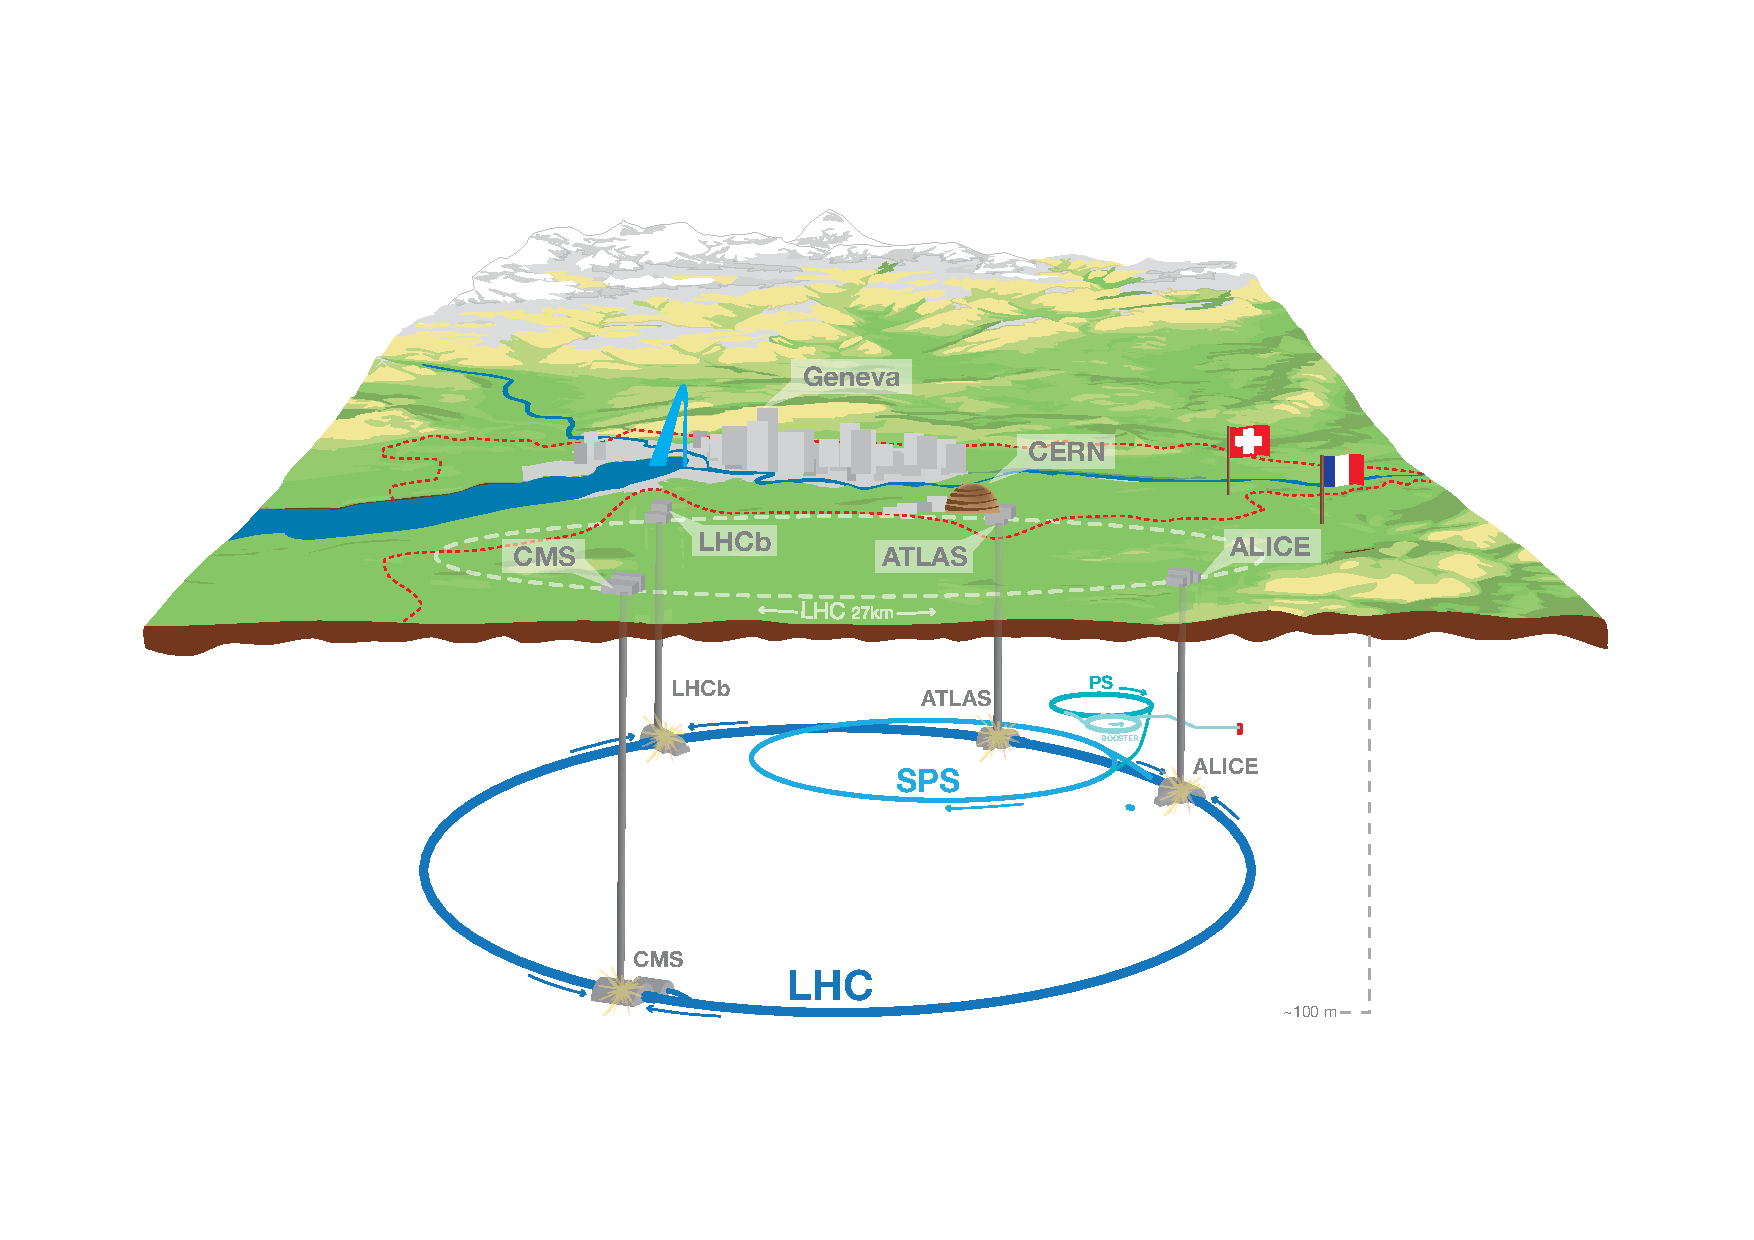
\includegraphics[width=16cm]{fig/Intro/LHCoverview.pdf}
\caption[LHC 加速器の概観]{LHC 加速器の概観\cite{cern_general_photo}。スイスとフランスの国境をまたがって、周長26.7 kmの円形加速器が設置されている。}
\label{LHCoverview}
\end{figure}

図\ref{ATLASdetector}にATLAS検出器の全体像を示す。ATLAS検出器は複数の検出器で構成された大型汎用検出器で、内部飛跡検出器、カロリメーター、ミューオンスペクトロメーターという3つの検出器群で構成される。最内層に設置された内部飛跡検出器は衝突点で生じた荷電粒子の飛跡を再構成し、運動量を測定する。その外側に設置されたカロリメーターは電子、光子、ハドロンを検出しそのエネルギーを測定する。最外層に設置されたミューオンスペクトロメーターは内側の検出器を透過してきたミューオンを捉え、その運動量を測定する。これらの検出器で測定された信号をイベントごとに集約することで、陽子陽子衝突で生じた事象を再構成し、物理解析を行なっている。

\begin{figure} 
    \centering
    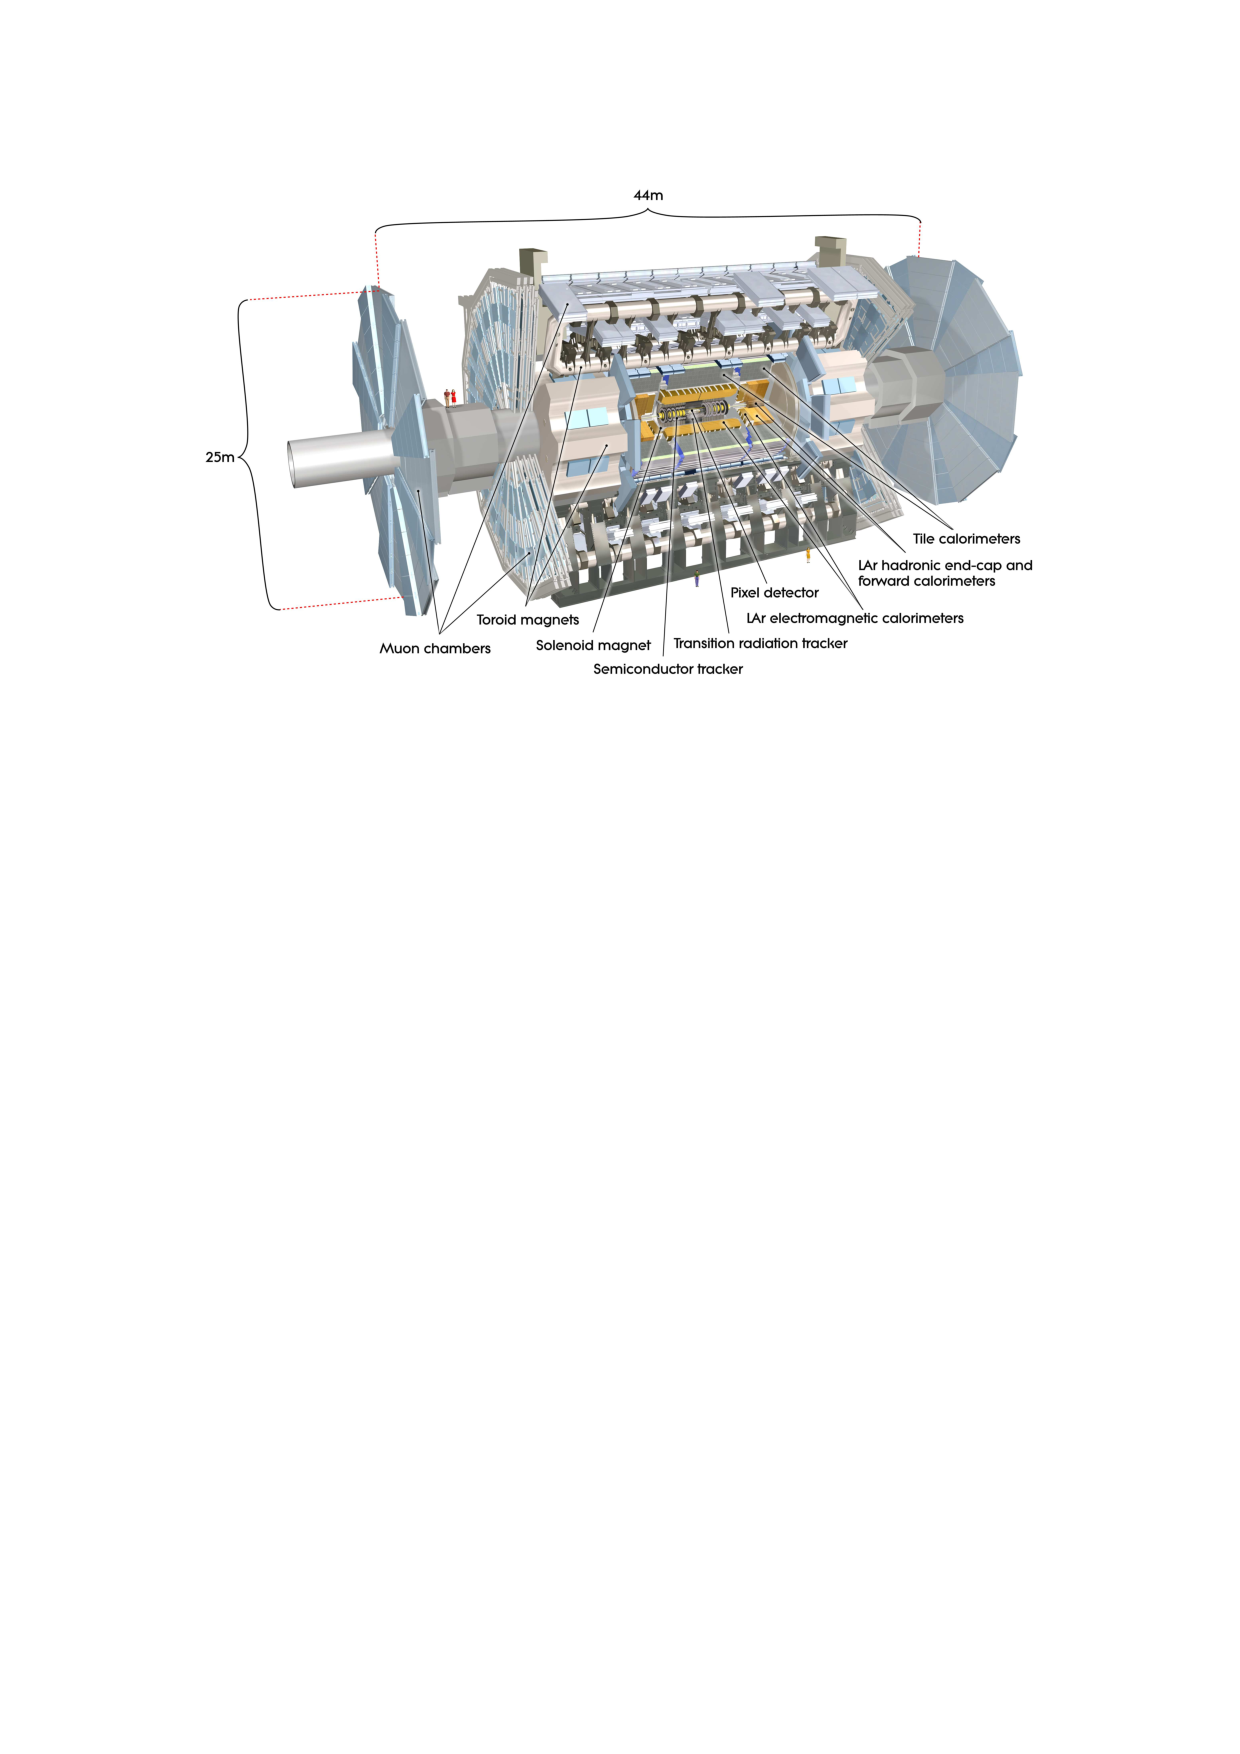
\includegraphics[width=16cm]{fig/Intro/ATLASdetector.pdf}
    \caption[ATLAS検出器の概要]{ATLAS検出器の概要図\cite{JINST:2008}。複数の検出機で構成された大型汎用検出器で、その長さは44 m、直径は25 mに及ぶ。内側から内部飛跡検出器、カロリーメーター、ミューオンスペクトロメーターという3つの検出器群で構成される。}
    \label{ATLASdetector}
\end{figure}

LHC加速器内部では、陽子はおよそ$10 ^ {11}$個ずつの束にまとめられ、陽子バンチを形成する。陽子バンチはLHCを周回しながら、最大エネルギー7.0 TeVまで加速され、それぞれの衝突点において40 MHzの頻度で交差する。
1回のバンチ交差で発生した大量の崩壊粒子は、それぞれの検出器にヒット信号を残す。それにより生じる情報量は1回の陽子衝突あたり約2 MByte程度である。これは1秒間に約80 TBpsのデータ量に相当し、その全てをストレージに転送し、保存することは技術的に不可能である。一方、陽子陽子衝突で生じるほとんどの事象は移行運動量がハドロンスケール程度の非弾性散乱で、エネルギーフロンティア物理の観点からは興味の薄いものである\footnote{超対称性で予言される新粒子やヒッグス粒子の断面積は、陽子陽子衝突の全断面積より$\mathcal{O}(10^{10})$程度小さい。}。

そこでATLAS実験では莫大な背景事象の中から、興味のある事象のみを高速で選別するトリガーシステムを採用している。ATLASのトリガーは2段階で構成されており、本研究で取り扱う2029年以降のシステムでは、ハードウェアで構成される初段トリガーで事象レートを40 MHzから1 MHzに、ソフトウェアで構成される後段トリガーで1 MHzから10 kHzまで選別する。トリガーシステムで選択されなかったデータは2度と取り戻すことができなない。そのため、物理的に興味の深い事象を確実に補足し、そうでないものを効率的に排除する精度の高いトリガーシステムを実現することは、物理プログラム成功のための必要条件といえる。
% \begin{figure} 
%     \centering
%     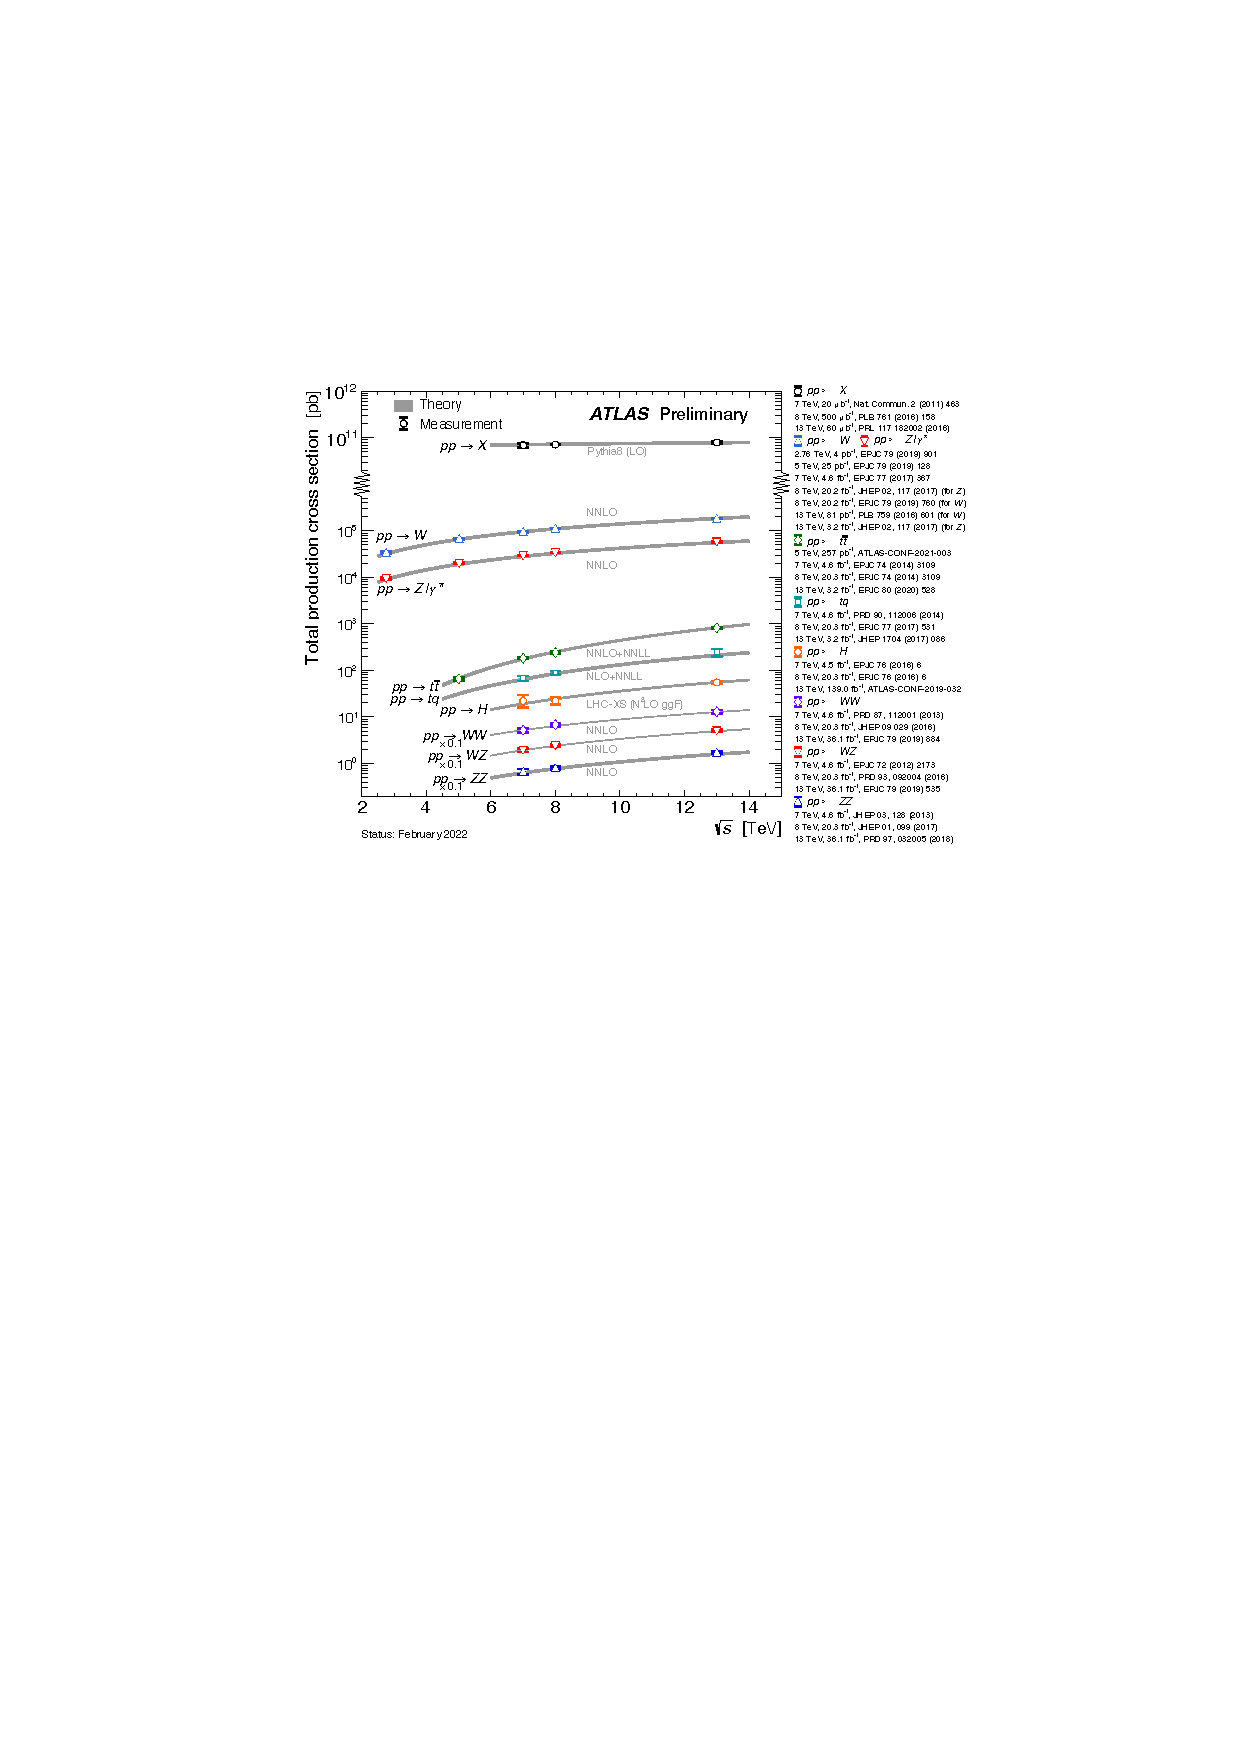
\includegraphics[width=16cm]{fig/Intro/LHCcrosssection.pdf}
%     \caption[陽子陽子衝突における各反応事象の断面積]{陽子陽子衝突における各反応事象の断面積 \cite{atlas_phys_pub_hllhc}}
%     \label{LHCcrosssection}
% \end{figure}


\section{高輝度LHC-ATLAS実験に向けたPhase-\two アップグレード}
\label{sec_intro_phase2upgrade}

\begin{figure} 
\centering
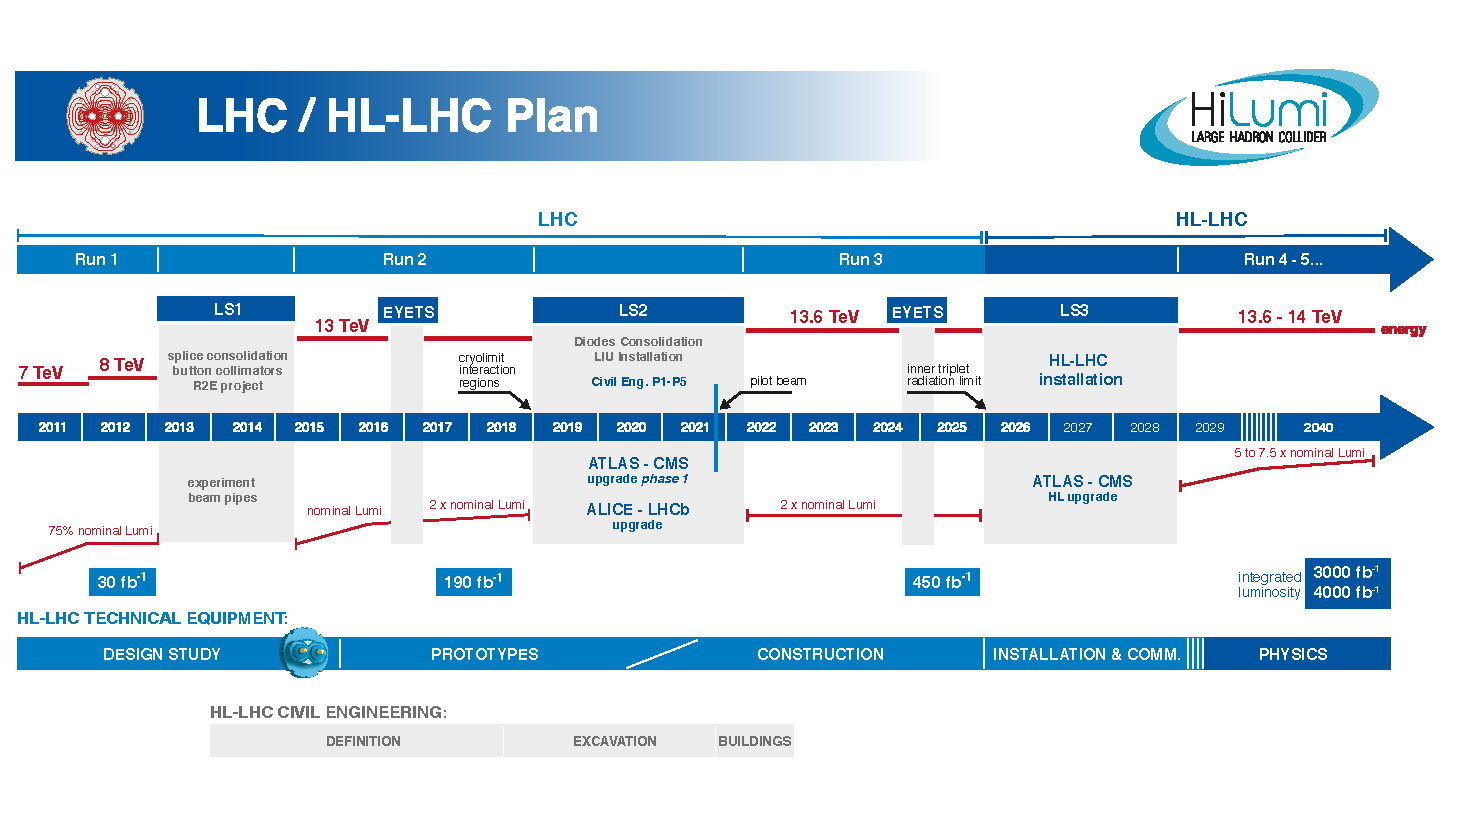
\includegraphics[width=16cm]{fig/Intro/LHCschedule.pdf}
\caption[LHC実験のスケージュール]{LHC実験のスケジュール\cite{cern_hllhc_industry}。LHC実験は2010年に本格的に稼働を開始し、2024年現在ではRun 3が進行中である。2026年から高輝度LHC実験に向けた装置の設置が始まり、2029年から運転が開始される。}
\label{LHCschedule}
\end{figure}

図\ref{LHCschedule}にLHCの運転スケジュールを示す。LHC実験は2010年から本格的に稼働を開始し、2024年現在では第三期運転 (Run 3) が進行中である。Run 3では2025年までに積分ルミノシティにして累計450 $\mathrm{fb}^{-1}$の統計量が蓄積されることが予定されている。その後、3年間のLong Shutdown (LS3) を経て、LHC加速器は高輝度化のため大幅にアプグレードされる。瞬間最高ルミノシティは現在の$2\times10^{34}\,\mathrm{cm}^{-2}\mathrm{s}^{-1}$から5 $\sim$ 7.5$\times10^{34}\,\mathrm{cm}^{-2}\mathrm{s}^{-1}$に増強され、2040年の実験終了までに蓄積される統計量は3000  $\sim$ 4000 $\mathrm{fb}^{-1}$に達する。これにより、新物理探索や標準模型の精密測定に対する感度は大きく向上することが期待される。

一方で、瞬間ルミノシティの増加に伴い、一回のバンチ交差ごとに発生する陽子陽子衝突数 (パイルアップ) が増え、背景事象が大幅に増加する。これに対応するために、高輝度LHC-ATLAS実験では検出器、データ収集システム、トリガーシステムが大幅にアップグレードされる。この一連のアップグレードをPhase-\two アップグレードと呼ぶ。Phase-\two アップグレードでは、内部飛跡検出器が全てシリコン検出器に置き換えられるほか、初段トリガーレートは100 kHzから1 MHzに、初段トリガーレイテンシーは2.5 $\mu\mathrm{s}$から 10 $\mu\mathrm{s}$に拡張される。これに伴って、各検出器のエレクトロニクスシステムの多くがアップグレードされる。

エンドキャップ部\footnote{ATLAS検出器では円筒の側面部分をバレル、底面部分をエンドキャップと呼ぶ。詳細は\ref{subsec_ATLAScordination}節で述べる。}初段ミューオントリガーを担当するThin Gap Chamber (TGC) 検出器でも一部を除いたすべてのエレクトロニクスが刷新される。TGC検出器信号のデジタル化および陽子バンチ交差とのタイミング同期を担当する前段回路は、FPGAを搭載したものへ置き換えられる。前段回路からのヒットデータをもとにトリガー判定を行う後段回路は、大規模FPGAとSystem on Chip (SoC)、双方向で2 Tbpsの大規模光I/O、を搭載したものへ置き換えられる。


% 図\ref{Ptthreshold}に、レプトントリガーシステム (特に、電子やミューオンの横方向運動量をもとに閾値を設定するシングルレプトントリガー) のアップグレードが与える物理探索感度への影響を示す。現行のレプトンの運動量分解能や信号転送レートを維持したまま、信号事象や背景事象が増加すると、閾値を超えるレプトンの数が読み出し能力を超えるため、レプトンの横方向運動量閾値を50 GeV程度まで上げなくてはならない。対して、トリガーシステムをアップグレードしてシングルレプトンの運動量分解能を向上させ、読み出し能力を増強することができれば、横方向運動量閾値を20 GeVまで低く抑えることができる。これにより、例えば終状態に低運動量レプトンが生成される縮退したSUSY粒子の崩壊事象へのアクセプタンスは、約4倍に増幅されること見込まれる。

% \begin{figure} 
% \centering
% 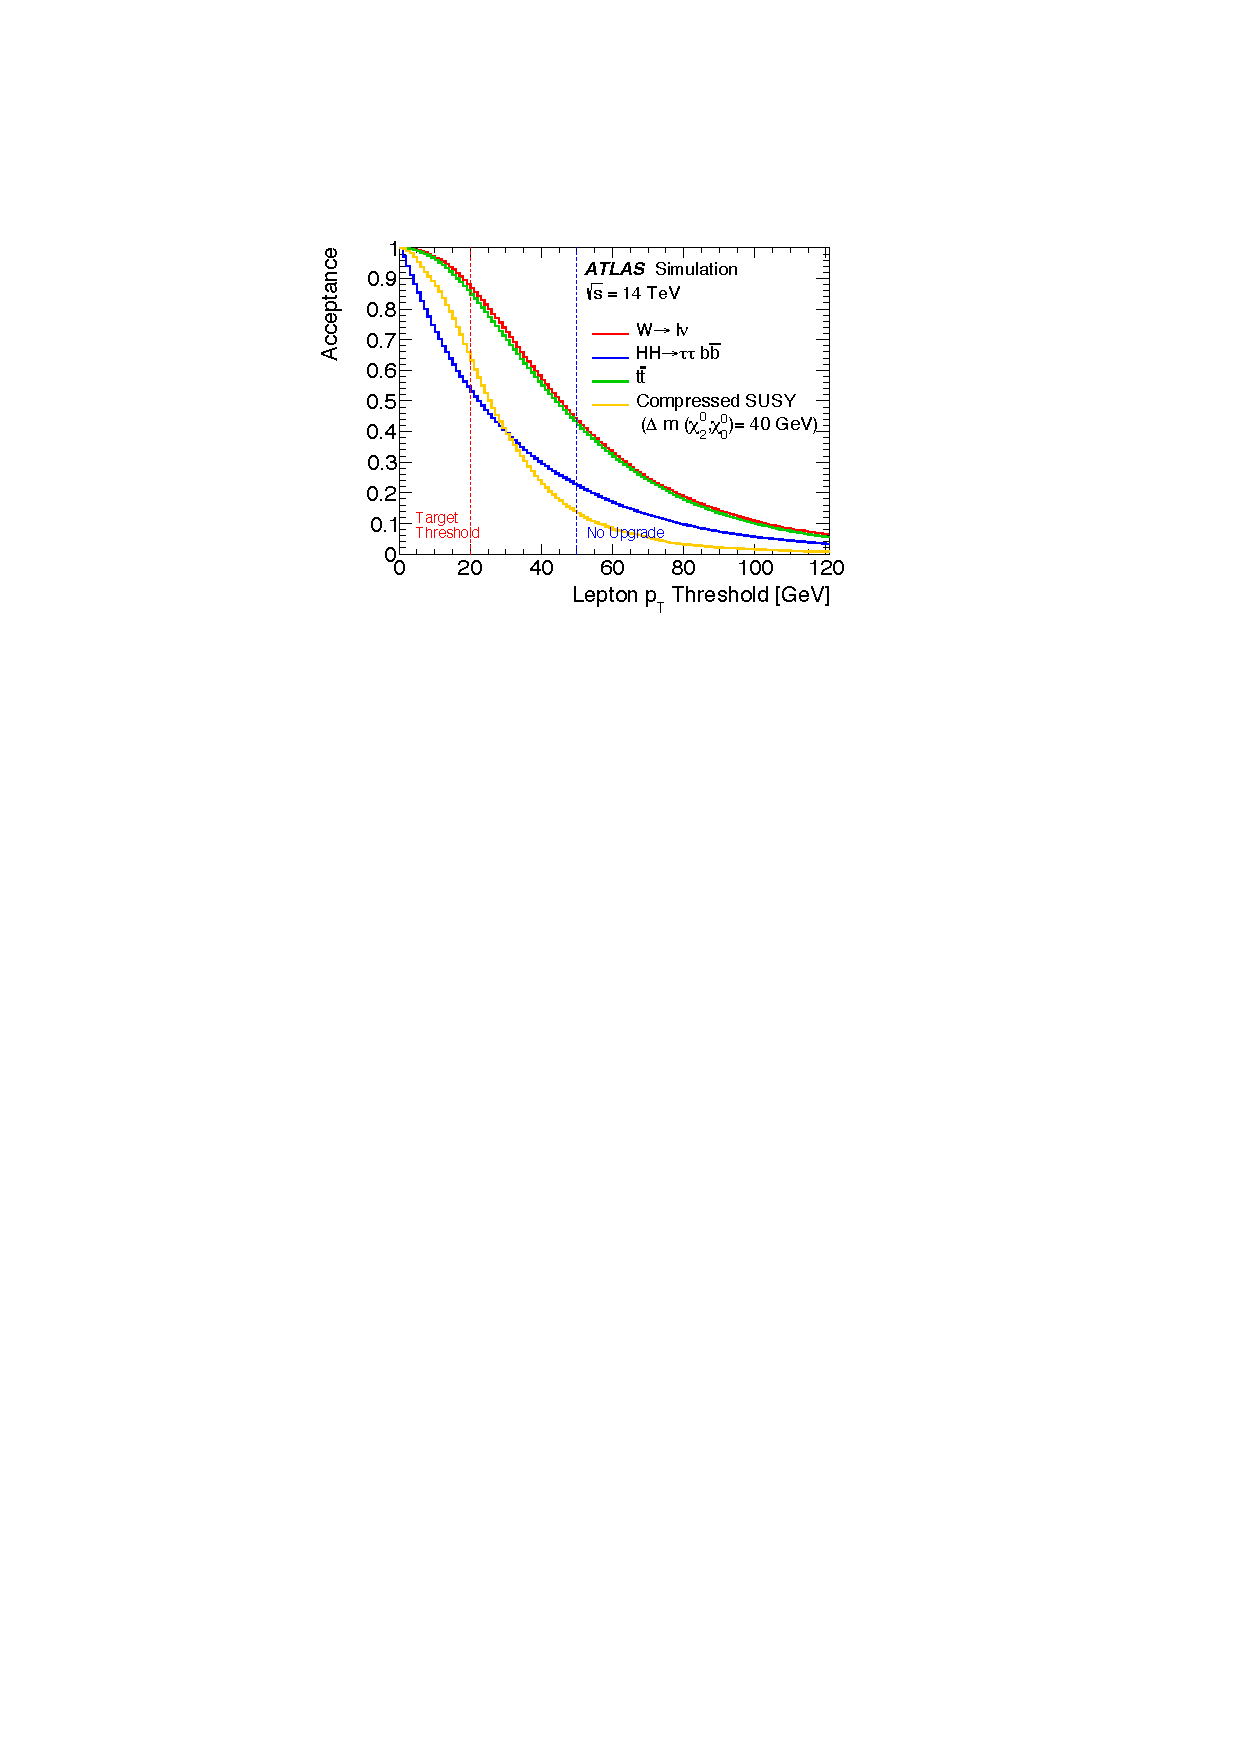
\includegraphics[width=16cm]{fig/Intro/Ptthreshold.pdf}
% \caption{レプトントリガーシステムのアップグレードが与える物理探索感度への影響\cite{tdr_phase2tdaq_2017020}。phase\two アップグレードにより、レプトンの横方向運動量閾値を50 GeVから20 GeVまで低く抑えることが可能となり、これによって興味のある物理事象へのアクセプタンスは大幅に向上することが見込まれる。}
% \label{Ptthreshold}
% \end{figure}


\section{本論文の目的・内容と構成}
\label{sec_intro_purpose}

本研究は、高輝度LHC-ATLAS実験に向けて、TGC検出器の後段回路に実装されるトリガー論理回路を完成させることを目的とする。そのために、まずトリガー回路を後段回路全体ファームウェアへと統合し、実機上で動作させるための準備を整える。次に、実装したトリガー回路の動作検証および性能評価に向けて、実機を用いたシングルボード試験システムを開発し、ミューオン飛跡のシミュレーションデータに対するトリガー効率を測定することで、トリガー回路が期待される性能を有しているか検証する。
また、本研究では多くの要素技術を共有する課題として、前段回路に対する品質保証試験の開発にも取り組む。これにより、2024年から開始される1500枚に及ぶ前段回路の量産に向けて必要不可欠なインフラを構築する。

これらの開発研究を通じて、本研究は将来の高エネルギー実験に幅広い応用が期待される、高速FPGAやSoCを活用した次世代型の検証モデルを確立した。

本論文の構成は以下の通りである。第\ref{chap_TGC}章では高輝度LHC-ATLAS実験に向けたTGC検出器システムのアップグレードについて説明し、各エレクトロニクスの役割を紹介する。第\ref{chap_TriggerIntegration}章では高輝度LHC-ATLAS実験でのエンドキャップ部ミューオントリガーロジックの詳細を説明し、トリガー回路の統合について述べる。第\ref{chap_TriggerTest}章では、トリガー論理回路の性能評価のために開発したシングルボード試験システムと、それを用いて行った試験の結果を述べる。第\ref{chap_QAQC}章では前段回路の量産に向けた、品質保証試験システムの設計・開発・実装について説明する。最後に\ref{chap_conclusion}章で本研究のまとめと今後の展望について述べる。